\documentclass{article}
\usepackage{tikz-qtree}
\usepackage{xcolor}
\usepackage{listings}

\lstset{
    language=C++,
    basicstyle=\ttfamily,
    keywordstyle=\color{blue},
    stringstyle=\color{red},
    commentstyle=\color{green!70!black},
    showstringspaces=false,
    breaklines=true,
    frame=tb,
    numbers=left,
    numberstyle=\tiny,
    numbersep=5pt,
    tabsize=2
}
\title{7. Uebungszettel}
\author{Steinbock, Gottlebe}

\begin{document}
\maketitle


\section*{1. Heaps (a)}
%%%%%%%%%%%%%%%%%%%%%%%%%%%%%%%%%%%%%%%%%%%%%%%%%%%%%%%%%%%%%%%%%%%%%%%%%%%%%%%%%%%%%%%%%%%%%%
\centering
\begin{minipage}{0.3\textwidth}
    \centering
    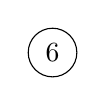
\begin{tikzpicture}
        \tikzset{every tree node/.style={minimum width=1.5em,draw,circle},
            blank/.style={draw=none},
            edge from parent/.style=
                {draw, edge from parent path={(\tikzparentnode) -- (\tikzchildnode)}},
            level distance=1.5cm}
        \Tree [.6 ]
    \end{tikzpicture}
\end{minipage}\hfill
\begin{minipage}{0.3\textwidth}
    \centering
    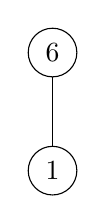
\begin{tikzpicture}
        \tikzset{every tree node/.style={minimum width=1.5em,draw,circle},
            blank/.style={draw=none},
            edge from parent/.style=
                {draw, edge from parent path={(\tikzparentnode) -- (\tikzchildnode)}},
            level distance=1.5cm}
        \Tree [.6 [.1 ]]
    \end{tikzpicture}
\end{minipage}\hfill
\begin{minipage}{0.3\textwidth}
    \centering
    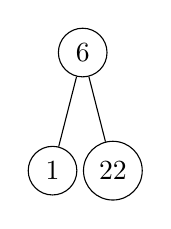
\begin{tikzpicture}
        \tikzset{every tree node/.style={minimum width=1.5em,draw,circle},
            blank/.style={draw=none},
            edge from parent/.style=
                {draw, edge from parent path={(\tikzparentnode) -- (\tikzchildnode)}},
            level distance=1.5cm}
        \Tree [.6 [.1 ] [.22 ]]
    \end{tikzpicture}
\end{minipage}
\vspace{1cm}

%%%%%%%%%%%%%%%%%%%%%%%%%%%%%%%%%%%%%%%%%%%%%%%%%%%%%%%%%%%%%%%%%%%%%%%%%%%%%%%%%%%%%%%%%%%%%%

\begin{minipage}{0.3\textwidth}
    \centering
    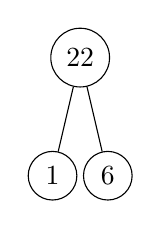
\begin{tikzpicture}
        \tikzset{every tree node/.style={minimum width=1.5em,draw,circle},
            blank/.style={draw=none},
            edge from parent/.style=
                {draw, edge from parent path={(\tikzparentnode) -- (\tikzchildnode)}},
            level distance=1.5cm}
        \Tree
        [.22
                [.1
                ]
                [.6
                ]
        ]
    \end{tikzpicture}
\end{minipage}\hfill
\begin{minipage}{0.3\textwidth}
    \centering
    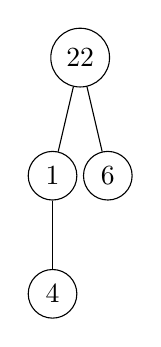
\begin{tikzpicture}
        \tikzset{every tree node/.style={minimum width=1.5em,draw,circle},
            blank/.style={draw=none},
            edge from parent/.style=
                {draw, edge from parent path={(\tikzparentnode) -- (\tikzchildnode)}},
            level distance=1.5cm}
        \Tree
        [.22
                [.1
                        [.4
                        ]
                ]
                [.6
                ]
        ]
    \end{tikzpicture}
\end{minipage}\hfill
\begin{minipage}{0.3\textwidth}
    \centering
    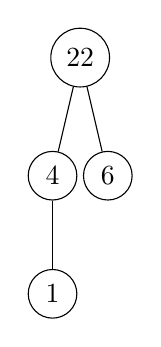
\begin{tikzpicture}
        \tikzset{every tree node/.style={minimum width=1.5em,draw,circle},
            blank/.style={draw=none},
            edge from parent/.style=
                {draw, edge from parent path={(\tikzparentnode) -- (\tikzchildnode)}},
            level distance=1.5cm}
        \Tree
        [.22
                [.4
                        [.1
                        ]
                ]
                [.6
                ]
        ]
    \end{tikzpicture}
\end{minipage}

\vspace{1cm}

%%%%%%%%%%%%%%%%%%%%%%%%%%%%%%%%%%%%%%%%%%%%%%%%%%%%%%%%%%%%%%%%%%%%%%%%%%%%%%%%%%%%%%%%%%%%%%

\begin{minipage}{0.3\textwidth}
    \centering
    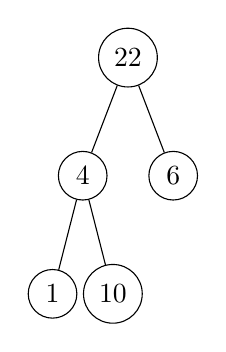
\begin{tikzpicture}
        \tikzset{every tree node/.style={minimum width=1.5em,draw,circle},
            blank/.style={draw=none},
            edge from parent/.style=
                {draw, edge from parent path={(\tikzparentnode) -- (\tikzchildnode)}},
            level distance=1.5cm}
        \Tree
        [.22
                [.4
                        [.1
                        ]
                        [.10
                        ]
                ]
                [.6
                ]
        ]
    \end{tikzpicture}
\end{minipage}\hfill
\begin{minipage}{0.3\textwidth}
    \centering
    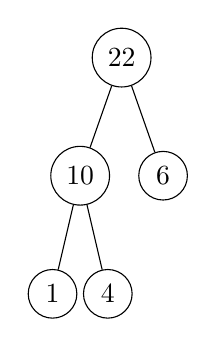
\begin{tikzpicture}
        \tikzset{every tree node/.style={minimum width=1.5em,draw,circle},
            blank/.style={draw=none},
            edge from parent/.style=
                {draw, edge from parent path={(\tikzparentnode) -- (\tikzchildnode)}},
            level distance=1.5cm}
        \Tree
        [.22
                [.10
                        [.1
                        ]
                        [.4
                        ]
                ]
                [.6
                ]
        ]
    \end{tikzpicture}
\end{minipage}\hfill
\begin{minipage}{0.3\textwidth}
    \centering
    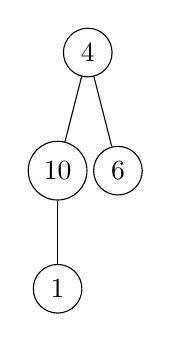
\begin{tikzpicture}
        \tikzset{every tree node/.style={minimum width=1.5em,draw,circle},
            blank/.style={draw=none},
            edge from parent/.style=
                {draw, edge from parent path={(\tikzparentnode) -- (\tikzchildnode)}},
            level distance=1.5cm}
        \Tree
        [.4
                [.10
                        [.1
                        ]
                ]
                [.6
                ]
        ]
    \end{tikzpicture}
\end{minipage}
\vspace{1cm}

%%%%%%%%%%%%%%%%%%%%%%%%%%%%%%%%%%%%%%%%%%%%%%%%%%%%%%%%%%%%%%%%%%%%%%%%%%%%%%%%%%%%%%%%%%%%%%

\begin{minipage}{0.3\textwidth}
    \centering
    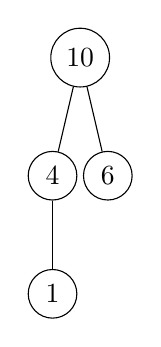
\begin{tikzpicture}
        \tikzset{every tree node/.style={minimum width=1.5em,draw,circle},
            blank/.style={draw=none},
            edge from parent/.style=
                {draw, edge from parent path={(\tikzparentnode) -- (\tikzchildnode)}},
            level distance=1.5cm}
        \Tree
        [.10
                [.4
                        [.1
                        ]
                ]
                [.6
                ]
        ]
    \end{tikzpicture}
\end{minipage}\hfill
\begin{minipage}{0.3\textwidth}
    \centering
    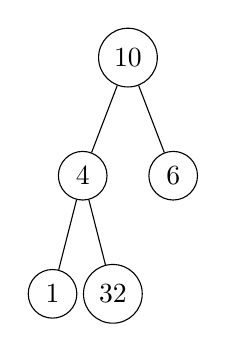
\begin{tikzpicture}
        \tikzset{every tree node/.style={minimum width=1.5em,draw,circle},
            blank/.style={draw=none},
            edge from parent/.style=
                {draw, edge from parent path={(\tikzparentnode) -- (\tikzchildnode)}},
            level distance=1.5cm}
        \Tree
        [.10
                [.4
                        [.1
                        ]
                        [.32
                        ]
                ]
                [.6
                ]
        ]
    \end{tikzpicture}
\end{minipage}\hfill
\begin{minipage}{0.3\textwidth}
    \centering
    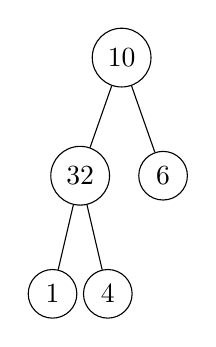
\begin{tikzpicture}
        \tikzset{every tree node/.style={minimum width=1.5em,draw,circle},
            blank/.style={draw=none},
            edge from parent/.style=
                {draw, edge from parent path={(\tikzparentnode) -- (\tikzchildnode)}},
            level distance=1.5cm}
        \Tree
        [.10
                [.32
                        [.1
                        ]
                        [.4
                        ]
                ]
                [.6
                ]
        ]
    \end{tikzpicture}
\end{minipage}
\vspace{1cm}

%%%%%%%%%%%%%%%%%%%%%%%%%%%%%%%%%%%%%%%%%%%%%%%%%%%%%%%%%%%%%%%%%%%%%%%%%%%%%%%%%%%%%%%%%%%%%%

\begin{minipage}{0.3\textwidth}
    \centering
    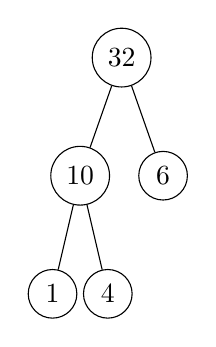
\begin{tikzpicture}
        \tikzset{every tree node/.style={minimum width=1.5em,draw,circle},
            blank/.style={draw=none},
            edge from parent/.style=
                {draw, edge from parent path={(\tikzparentnode) -- (\tikzchildnode)}},
            level distance=1.5cm}
        \Tree
        [.32
                [.10
                        [.1
                        ]
                        [.4
                        ]
                ]
                [.6
                ]
        ]
    \end{tikzpicture}
\end{minipage}\hfill
\begin{minipage}{0.3\textwidth}
    \centering
    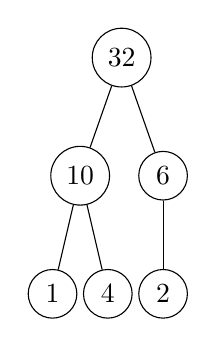
\begin{tikzpicture}
        \tikzset{every tree node/.style={minimum width=1.5em,draw,circle},
            blank/.style={draw=none},
            edge from parent/.style=
                {draw, edge from parent path={(\tikzparentnode) -- (\tikzchildnode)}},
            level distance=1.5cm}
        \Tree
        [.32
                [.10
                        [.1
                        ]
                        [.4
                        ]
                ]
                [.6
                        [.2
                        ]
                ]
        ]
    \end{tikzpicture}
\end{minipage}\hfill
\begin{minipage}{0.3\textwidth}
    \centering
    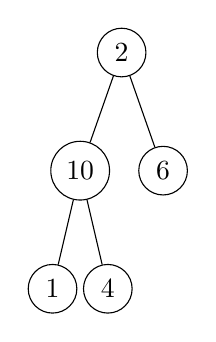
\begin{tikzpicture}
        \tikzset{every tree node/.style={minimum width=1.5em,draw,circle},
            blank/.style={draw=none},
            edge from parent/.style=
                {draw, edge from parent path={(\tikzparentnode) -- (\tikzchildnode)}},
            level distance=1.5cm}
        \Tree
        [.2
                [.10
                        [.1
                        ]
                        [.4
                        ]
                ]
                [.6
                ]
        ]
    \end{tikzpicture}
\end{minipage}
\vspace{1cm}

%%%%%%%%%%%%%%%%%%%%%%%%%%%%%%%%%%%%%%%%%%%%%%%%%%%%%%%%%%%%%%%%%%%%%%%%%%%%%%%%%%%%%%%%%%%%%%

\begin{minipage}{0.3\textwidth}
    \centering
    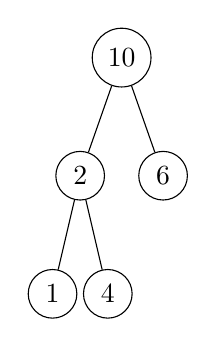
\begin{tikzpicture}
        \tikzset{every tree node/.style={minimum width=1.5em,draw,circle},
            blank/.style={draw=none},
            edge from parent/.style=
                {draw, edge from parent path={(\tikzparentnode) -- (\tikzchildnode)}},
            level distance=1.5cm}
        \Tree
        [.10
                [.2
                        [.1
                        ]
                        [.4
                        ]
                ]
                [.6
                ]
        ]
    \end{tikzpicture}
\end{minipage}\hfill
\begin{minipage}{0.3\textwidth}
    \centering
    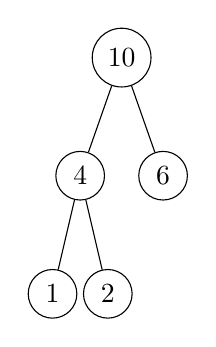
\begin{tikzpicture}
        \tikzset{every tree node/.style={minimum width=1.5em,draw,circle},
            blank/.style={draw=none},
            edge from parent/.style=
                {draw, edge from parent path={(\tikzparentnode) -- (\tikzchildnode)}},
            level distance=1.5cm}
        \Tree
        [.10
                [.4
                        [.1
                        ]
                        [.2
                        ]
                ]
                [.6
                ]
        ]
    \end{tikzpicture}
\end{minipage}\hfill
\begin{minipage}{0.3\textwidth}
    \centering
    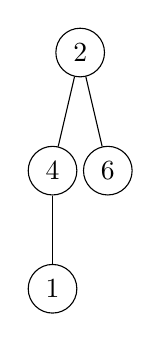
\begin{tikzpicture}
        \tikzset{every tree node/.style={minimum width=1.5em,draw,circle},
            blank/.style={draw=none},
            edge from parent/.style=
                {draw, edge from parent path={(\tikzparentnode) -- (\tikzchildnode)}},
            level distance=1.5cm}
        \Tree
        [.2
                [.4
                        [.1
                        ]
                ]
                [.6
                ]
        ]
    \end{tikzpicture}
\end{minipage}
\vspace{1cm}

%%%%%%%%%%%%%%%%%%%%%%%%%%%%%%%%%%%%%%%%%%%%%%%%%%%%%%%%%%%%%%%%%%%%%%%%%%%%%%%%%%%%%%%%%%%%%%

\begin{minipage}{0.45\textwidth}
    \centering
    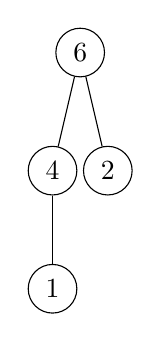
\begin{tikzpicture}
        \tikzset{every tree node/.style={minimum width=1.5em,draw,circle},
            blank/.style={draw=none},
            edge from parent/.style=
                {draw, edge from parent path={(\tikzparentnode) -- (\tikzchildnode)}},
            level distance=1.5cm}
        \Tree
        [.6
                [.4
                        [.1
                        ]
                ]
                [.2
                ]
        ]
    \end{tikzpicture}
\end{minipage}\hfill

\section*{1. Heaps (b)}

Die $\Omega$-Notation gibt eine untere Schranke für die Laufzeit eines Algorithmus an. Wenn wir sagen, dass ein Algorithmus eine Laufzeit von $\Omega (n \log n)$ hat, bedeutet das, dass der Algorithmus nicht schneller als $n \log n$ ausgeführt werden kann, für große Werte von $n$.

\vspace*{0.5cm}

Vergleichsbasiertes Sortieren hat eine untere Schranke von $\Omega (n \log n)$. Das bedeutet, dass jeder vergleichsbasierte Sortieralgorithmus mindestens $n \log n$ Vergleiche benötigt, um eine Liste von $n$ Elementen zu sortieren, im schlimmsten Fall.

\vspace*{0.5cm}

Nun betrachten wir eine Sequenz von n insert-Operationen und $n$ extractMax-Operationen auf einer vergleichsbasierten Datenstruktur. Jede insert-Operation fügt ein Element in die Datenstruktur ein und jede extractMax-Operation entfernt das größte Element aus der Datenstruktur. Nachdem alle insert-Operationen ausgeführt wurden, sind alle Elemente in der Datenstruktur und die extractMax-Operationen entfernen die Elemente in absteigender Reihenfolge. Dies entspricht im Wesentlichen einem Sortierprozess.

\vspace*{0.5cm}

Da die Datenstruktur vergleichsbasiert ist, muss sie für jede insert- und extractMax-Operation Vergleiche durchführen, um das Element an der richtigen Stelle einzufügen bzw. das größte Element zu finden. Da wir insgesamt $2n$ Operationen durchführen ($n$ insert-Operationen und $n$ extractMax-Operationen) und jede Operation mindestens $\log n$ Vergleiche erfordert (da wir ein Element in einer sortierten Liste von $n$ Elementen einfügen bzw. das größte Element finden), haben wir insgesamt mindestens $2n \log n$ Vergleiche.

\vspace*{0.5cm}

Da $2n \log n = \Omega(n \log n)$ (da wir nur an der Größenordnung interessiert sind und konstante Faktoren ignorieren), haben wir gezeigt, dass eine Sequenz von $n$ insert-Operationen und $n$ extractMax-Operationen auf einer vergleichsbasierten Datenstruktur eine Gesamtlaufzeit von $\Omega(n \log n)$ hat.

\section*{2. Pointer und Referenzen (a)}

Ein Pointer ist eine Variable, die die Adresse (Speicherstelle) einer Variable speichert.

Eine Referenz ist ein zusätzlicher Name für eine Variable.

\section*{2. Pointer und Referenzen (b)}

Call-by-Reference ist eine Methode, die in einigen Programmiersprachen zur Übergabe von Argumenten an Funktionen verwendet wird. Bei dieser Methode wird eine Referenz auf die Originalvariable, anstatt deren Wert, an die Funktion übergeben. Dies ermöglicht es der Funktion, den Wert der Originalvariable zu ändern.

\vspace*{0.5cm}


\begin{lstlisting}[language=C++]
    #include <iostream>

    void aendern(int *ptr)
    {
        *ptr = 10;
    }
    
    int main()
    {
        int x = 5;
        std::cout << "Davor: " << x << std::endl;
        aendern(&x);
        std::cout << "Danach: " << x << std::endl;
    }
\end{lstlisting}

\section*{2. Pointer und Referenzen (c)}

\begin{lstlisting}[language=C++]
    void increase(int* aptr){
        (*aptr)++;
        }
\end{lstlisting}

\vspace*{0.5cm}


Spezifikation:

Die Funktion erhält einen Zeiger auf einen Integer-Wert (int* aptr) als Eingabe.

Sie erhöht den Wert, auf den der Zeiger zeigt, um eins.

Die Funktion hat keinen Rückgabewert (void).

\vspace*{0.5cm}

In der Regel spricht man von Call-by-Value, wenn der übergebene Wert in der Funktion nicht verändert wird und von Call-by-Reference, wenn der Originalwert modifiziert werden kann. In diesem Fall übergibt die Funktion den Speicherort (also den Zeiger) der zu ändernden Variable, nicht den Wert selbst. Das bedeutet, dass die Änderungen, die in der Funktion vorgenommen werden, sich auf die ursprüngliche Variable auswirken, auf die der Zeiger zeigt. Daher ist dies ein Fall von Call-by-Reference.

\section*{2. Pointer und Referenzen (d)}

\begin{lstlisting}[language=C++]
    #include <iostream>

    int summeZahlen()
    {
        int k;
        std::cout << "Geben Sie k an: ";
        std::cin >> k;

        int *arr = new int[k];

        for (int i = 0; i < k; ++i)
        {
            std::cout << "Geben Sie eine Zahl ein: ";
            std::cin >> arr[i];
        }

        int summe = 0;
        for (int i = 0; i < k; ++i)
        {
            summe += arr[i];
        }

        delete[] arr;

        return summe;
    }

    int main()
    {
        int summe = summeZahlen();
        std::cout << "Die Summe ist: " << summe << std::endl;
    }

\end{lstlisting}

\newpage

\section*{3. Noch mehr Pointer und Referenzen (a)}

\begin{table}[h]
    \centering
    \begin{tabular}{|c|c|c|}
        \hline
        \textbf{Adresse} & \textbf{Variable} & \textbf{Wert}              \\
        \hline
        0x16cf5af7c      & a                 & 42                         \\
        0x16cf5af78      & b                 & 6                          \\
        0x16cf5af70      & c                 & \&a 0x16cf5af7c            \\
        0x16cf5af68      & d                 & \&b 0x16cf5af78            \\
        0x16cf5af7c      & e                 & 42 (gleiche Adresse wie a) \\
        \hline
    \end{tabular}
    \caption{Speicheraufbau nach der ersten Änderung}
\end{table}

\begin{table}[h]
    \centering
    \begin{tabular}{|c|c|c|}
        \hline
        \textbf{Adresse} & \textbf{Variable} & \textbf{Wert}               \\
        \hline
        0x16cf5af7c      & a                 & 252                         \\
        0x16cf5af78      & b                 & 756                         \\
        0x16cf5af70      & c                 & \&a 0x16cf5af7c             \\
        0x16cf5af68      & d                 & 3                           \\
        0x16cf5af7c      & e                 & 252 (gleiche Adresse wie a) \\
        \hline
    \end{tabular}
    \caption{Speicheraufbau nach der zweiten Änderung}
\end{table}

\begin{table}[h]
    \centering
    \begin{tabular}{|c|c|c|}
        \hline
        \textbf{Adresse} & \textbf{Variable} & \textbf{Wert}              \\
        \hline
        0x16cf5af7c      & a                 & 14                         \\
        0x16cf5af78      & b                 & 7                          \\
        0x16cf5af70      & c                 & \&a 0x16cf5af7c            \\
        0x16cf5af68      & d                 & 3                          \\
        0x16cf5af7c      & e                 & 14 (gleiche Adresse wie a) \\
        \hline
    \end{tabular}
    \caption{Speicheraufbau nach der dritten Änderung}
\end{table}

\section*{3. Noch mehr Pointer und Referenzen (b)}

ref(a) ist eine Funktion, die eine Referenz auf a nimmt (also die Speicheradresse von a). Daher ist \&alpha gleich \&a und alpha gleich a. Nach dem Aufruf der Funktion wird der Wert von a um eins erhöht (wegen alpha++), deshalb ist a jetzt 15.

\vspace*{0.5cm}

val(a) ist eine Funktion, die den Wert von a nimmt, aber eine neue Kopie des Wertes erstellt (weil es Call-by-Value ist). Daher ist alpha gleich a, aber \&alpha ist nicht gleich \&a. Nach dem Aufruf der Funktion bleibt a 15, weil die Erhöhung von alpha nur auf die Kopie angewendet wird, nicht auf das Original a.

\vspace*{0.5cm}

func1(c) ist eine Funktion, die den Wert von c nimmt, der die Adresse von a ist. Daher ist alpha gleich c und \&alpha ist eine neue Speicheradresse (die Adresse des Zeigers selbst, nicht die Adresse, auf die er zeigt). Nach dem Aufruf der Funktion wird c verändert, weil alpha++ den Zeiger verschiebt, aber a bleibt unverändert.

\vspace*{0.5cm}

func2(c) ist eine Funktion, die den Wert von c nimmt, der die Adresse von a ist. Daher ist alpha gleich c und \&alpha ist eine neue Speicheradresse (die Adresse des Zeigers selbst, nicht die Adresse, auf die er zeigt). Nach dem Aufruf der Funktion wird der Wert von a erhöht (wegen (*alpha)++), deshalb ist a jetzt 16. Aber c bleibt unverändert, weil es immer noch auf die Adresse von a zeigt.

\section*{3. Noch mehr Pointer und Referenzen (c)}

Das Problem ist, dass a und e nicht als Zeiger definiert sind, sondern als int. Sie sind normale Integer-Variablen und haben keine Speicheradresse, auf die sie verweisen. Das Dereferenzieren von a und e ist daher nicht zulässig und führt zu einem Fehler.

\end{document}

